\chapter{Exploración Información-Teórica, Desafíos y Problemas Abiertos}%
\label{cha:exploración_información_teórica_desafíos_y_problemas_abiertos}

\lecture{21}{2020-08-07}{Information-Theoretic Exploration, Challenges and Open Problems}

\section{Exploración sin una función de recompensa}%
\label{sec:exploración_sin_una_función_de_recompensa}

Hay varios motivos para conseguir un comportamiento de esta manera:
\begin{itemize}
    \item Aprender habilidades sin supervisión y usarlas después para cumplir objetivos.
    \item Aprender sub-habilidades para usarlas en RL jerárquico.
    \item Explorar el espacio de los posibles comportamientos.
\end{itemize}

\subsection{Definiciones y conceptos de la teoría de la información}%
\label{sub:definiciones_y_conceptos_de_la_teoría_de_la_información}

\begin{itemize}
    \item $p(x)$: distribución.
    \item $H(p(x))=-E_{x\sim p(x)}[\log p(x)]$: entropía
    \item Información mutua, dice cuánto de dependientes son las dos variables. Es la
        identidad más importante de las tres:
        \begin{align}
            I(x;y)&=D_{KL}(p(x,y)||p(x)p(y))\\
                  &= E_{(x,y)\sim p(x,y)}\left[\log \frac{p(x,y)}{p(x)p(y)}  \right]\\
                  &= H(p(y)) - H(p(y|x))
        \end{align}
\end{itemize}

Cantidades de la teoría de la información en RL:
\begin{itemize}
    \item $\pi(s)$: distribución marginal de estados de la política $\pi$ 
    \item $H(\pi(s))$: cuantifica la cobertura de  $\pi(s)$.
    \item \textit{Empowerment}: la habilidad que tiene el agente de afectar al mundo, se calcula
        como:
        \begin{align}
            I(s_{t+1};a)=H(s_{t+1}-H(s_{t+1}|a_t))
        \end{align}
\end{itemize}

\subsection{Aprender sin una función de recompensa, completando objetivos}%
\label{sub:aprender_sin_una_función_de_recompensa_completando_objetivos}

En este caso, se tiene un estado inicial y se le dice al agente que tiene que llegar al estado
deseado interaccionando con el mundo. El agente construye una representación interna, mediante
un VAE por ejemplo.

\begin{center}
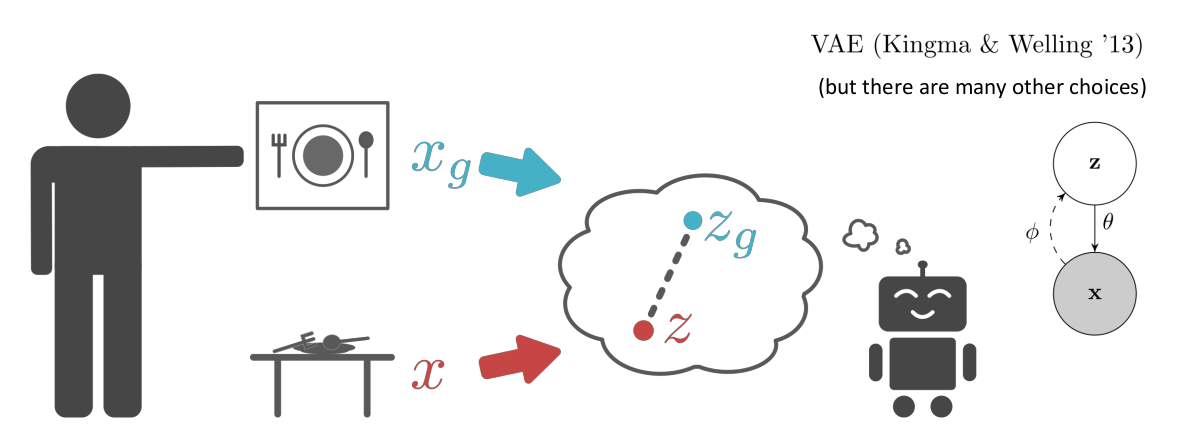
\includegraphics[width=.8\textwidth]{figures/2020-08-07-135150_1179x448_scrot.png}
\end{center}

Una forma de aprender sería que el agente intente llegar del estado inicial a otros estados
aleatorios, entrenando su política para alcanzar estos estados. Pero esto tiene el problema de
que no se explora el espacio de forma óptima, ya que el agente sólo explorará entornos
cercanos porque son los que su modelo generativo puede generar. Lo que hace que 'vaya en
círculos'.

En general, el algoritmo es así:
\begin{enumerate}
    \item Se propone un objetivo: $z_g\sim p(z), x_g\sim p_\theta (x_g|z_g)$
    \item Se intenta alcanzar el objetivo con $\pi(a|x,x_g)$, se llega a  $\overline{x}$.
    \item Se usan los datos para actualizar $\pi$.
    \item Se usan los datos para actualizar $p_\theta(x_g,z_g), q_\phi(z_g|x_g)$
\end{enumerate}

Pero se tiene que encontrar una forma de diversificar los objetivos. La clave está en
modificar el paso 4, de tal forma que se haga más énfasis en los estados nuevos. Por lo que
en vez de usar MLE estándar, se pasa a usar MLE ponderado:
\begin{align}
    \theta,\phi \gets arg\max_{\theta,\phi} E[w(\overline{x})\log p(\overline{x})]
\end{align}
Si se elige $w(\overline{x})=p_\theta(\overline{x})^\alpha\;\;\alpha\in [-1,0)$, la entropía
$H(p_\theta(x))$ se incrementa.

\begin{center}
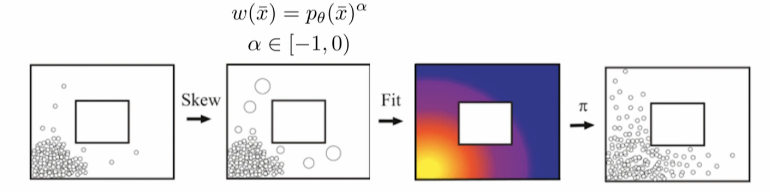
\includegraphics[width=.6\textwidth]{figures/2020-08-07-142207_770x193_scrot.png}
\end{center}

Esto hace que el objetivo sea maximizar $H(p(G))$. Pero por el otro lado, RL está entrenando
$\pi(a|S,G)$ para alcanzar  $G$, por lo que mientras $\pi$ va mejorando, el estado final $S$ se
va aproximando a $G$, lo que significa que $p(G|S)$ se va haciendo más determinista.

Por lo que el objetivo se puede expresar como $\max H(p(G))-H(p(G|S))$, lo que significa que es
la información mutua: $\max I(S;G)$.

\subsection{Mas allá del cubrimiento de estados: cubriendo el espacio de habilidades}%
\label{sub:mas_allá_del_cubrimiento_de_estados_cubriendo_el_espacio_de_habilidades}

Intuición: habilidades diferentes deben de visitar diferentes regiones del espacio de estados.

\begin{center}
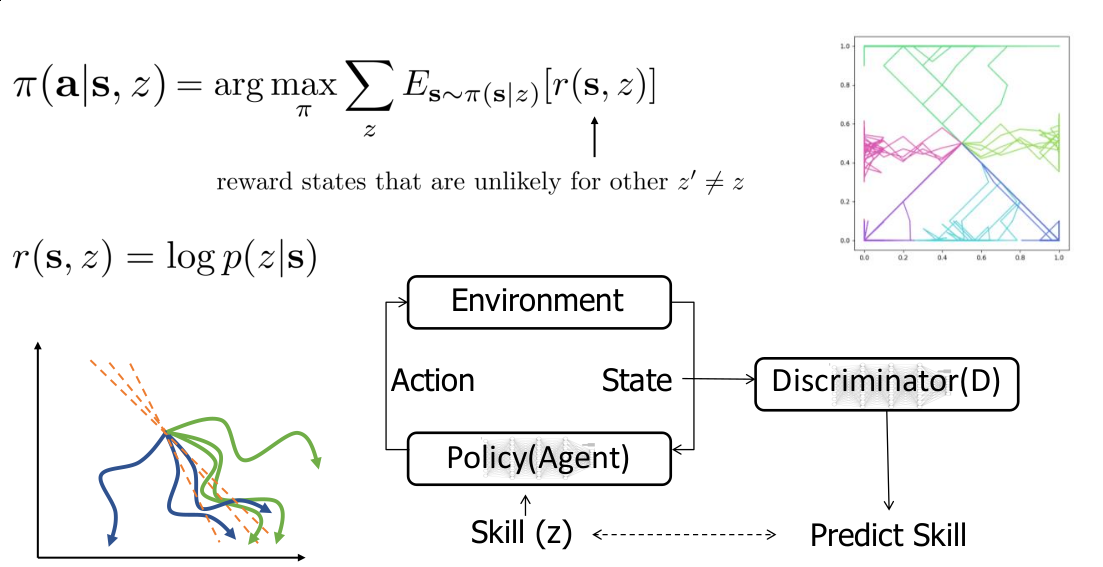
\includegraphics[width=.8\textwidth]{figures/2020-08-07-144241_1103x567_scrot.png}
\end{center}

Lo anterior equivale a maximizar la información mutua pero de $z$ y $s$ :
\begin{align}
    I(z,s)=H(z)-H(z|s)
\end{align}
El primer término es maximizado usando $p(z)$ y el segundo es minimizado mediante la
maximización de $\log p(z|s)$.

%\subsection{Uso de RL no supervisado para meta-learning}%
%\label{sub:uso_de_rl_no_supervisado_para_meta_learning}

\section{Desfíos en Deep Reinforcement Learning}%
\label{sec:desfíos_en_deep_reinforcement_learning}

Problemas en los algoritmos principales:
\begin{itemize}
    \item Estabilidad: convergencia. 
    \item Eficiencia: muestras necesarias.
    \item Generalización: después de la convergencia, generaliza?
\end{itemize}

Problemas con las asunciones:
\begin{itemize}
    \item RL provee de una buena formulación a problemas pero la pregunta es si esta formulación
        es la correcta.
    \item ¿De dónde viene el conocimiento?
\end{itemize}

Problemas con los hiperparámetros:
\begin{itemize}
    \item No se puede hacer un barrido de hiperparámetros en la vida real. Normalmente los
        parámetros obtenidos en simuladores no son representativos.
    \item Existen algoritmos que buscan una mejora de las propiedades de convergencia como
        TRPO u otros que ajustan adaptativamente sus hiperparámetros.
\end{itemize}

\subsection{Complejidad del muestreo}%
\label{sub:complejidad_del_muestreo}

\begin{center}
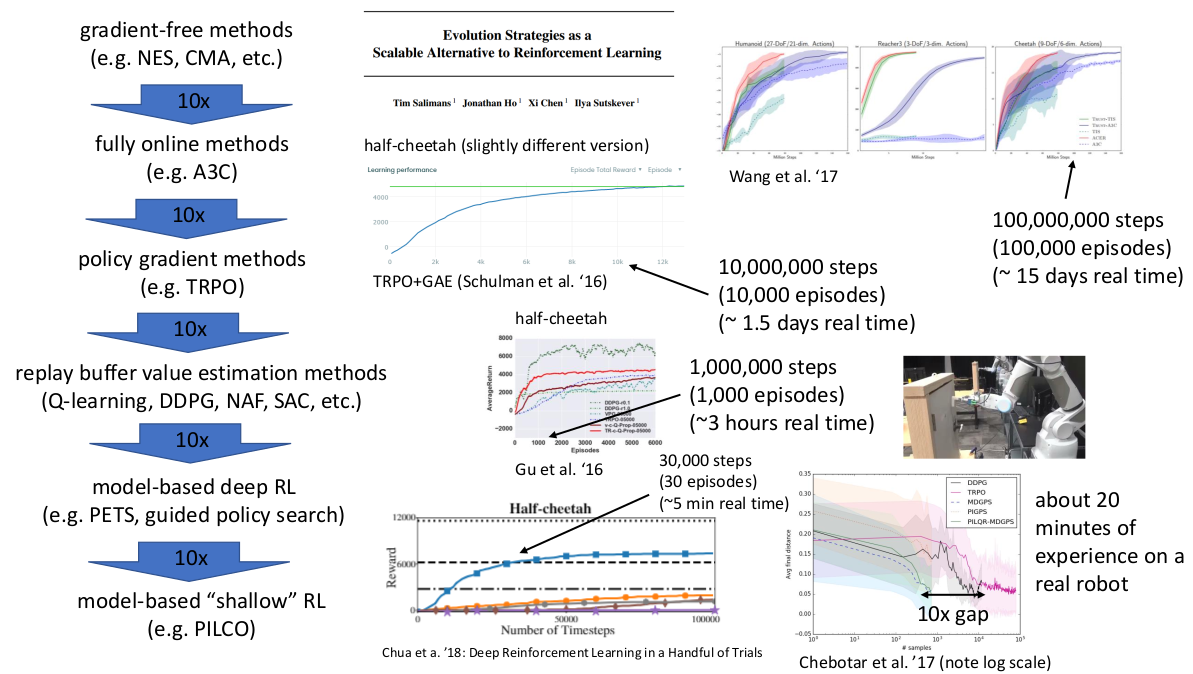
\includegraphics[width=.8\textwidth]{figures/2020-08-07-161110_1193x674_scrot.png}
\end{center}

\subsection{Escalado y generalización}%
\label{sub:escalado_y_generalización}

DL en el aprendizaje supervisado consigue resultados a grande escala, enfatiza la
diversidad y está evaluada en la generalización. Por otra parte, DRL es de escala pequeña y
enfatiza el dominio de una tarea evaluada, por lo que no hay generalización.
